\section{Compressed Sensing}
\label{s:introduction_cs}

Real world signals can be viewed as multidimensional vector and we know that image can be represented as
a matrix with pixel entries as each element. It can also be viewed as multidimensional vector
just by stacking the columns of the image matrix one after the other. In signal processing we measure
samples of the signal in order to reconstruct the original signal. For reconstruction of such signals we
consider linear measurement model
\begin{equation}
Ax = b
\label{1.1}
\end{equation}

\begin{tabular}{ll}
 where,& $A$ is the known measurement matrix of order $M \times N$ \\
      & $M$ is the number of rows or number of features \\
      & $N$ is the number of columns or number of unknowns \\
      & $b$ is the $M \times 1$ known vector called measurement vector. \\
      & \hspace{6mm} Each element of b vector is a measurement.\\ 
      & $x$ is the $N \times 1$ unknown vector which we want to reconstruct.\\
\end{tabular}
\\ \\This is our classical linear algebra problem which has three cases. 
\begin{itemize}
\item $M=N$ then $A$ is a square matrix and if A is non-singular then the system of equations has a
unique solution.

\item $M>N$ $A$ matrix is a rectangular matrix with the number of rows (or number of equations) is greater
than number of unknowns. Such systems are called Overdetermined systems and have no solution. Least Square 
method is one of the method for arriving at an approximate solution.

\item $M<N$ then $A$ matrix is a rectangular matrix with the number of rows smaller than the number of columns.
Then, the system of equation is called as Under determined system and has a whole subspace of solution.
\end{itemize}

\paragraph{}Suppose we have far fewer measurements than the number of  
features or unknowns i.e. $M<<N$. Compressed Sensing can then provide a solution if we know that the signal is sparse (\cite{david06}). 

\subsection{Sparsity}
\label{s:sparsity}

\paragraph{}With the success of image processing, where great advances in compression and estimation have come
from modeling images as sparse in a wavelet domain (JPEG 2000 standard), modeling signals in a sparse
basis has become a key area in signal processing. To illustrate this consider an $N$ dimensional vector
$y$ that can represented as $\Psi x$, where $\Psi$ is a $N \times N$ orthogonal matrix aka \emph{Basis Matrix} 
and $x \in R^N$ has $k$ non-zero entries. In this case we say that $x$ is $k$-sparse or $x$ is a k-sparse representation
of $y$ with respect to $\Psi$. The ratio $\alpha = k/N$ is called sparsity ratio of vector $x$.

\paragraph{}Sparsity is the fundamental criterion for compressed sensing to work. Most signals (or images) are 
sparse when represented in certain sparsifying bases. An advantage in knowing the sparse representation
of a signal is that the degree of freedom of signal the signal is reduced by a significant amount which leads to compression.
Compression gain is higher when sparsity ratio is smaller.

\paragraph{}Another important property of sparse signals is that it can be recovered in far less number of
measurements then it would be otherwise. This technique is called as \emph{Compressed Sensing or Compressive
sampling} was developed by \cite{Can106}, \cite{Can206}, \cite{david06} .

\paragraph{}The sampling of $y$ is represented as a linear transformation
 by a matrix $\Phi$  yielding a measurement vector $b = \Phi y$. 
\begin{figure}[!htbp]
  \begin{center}
      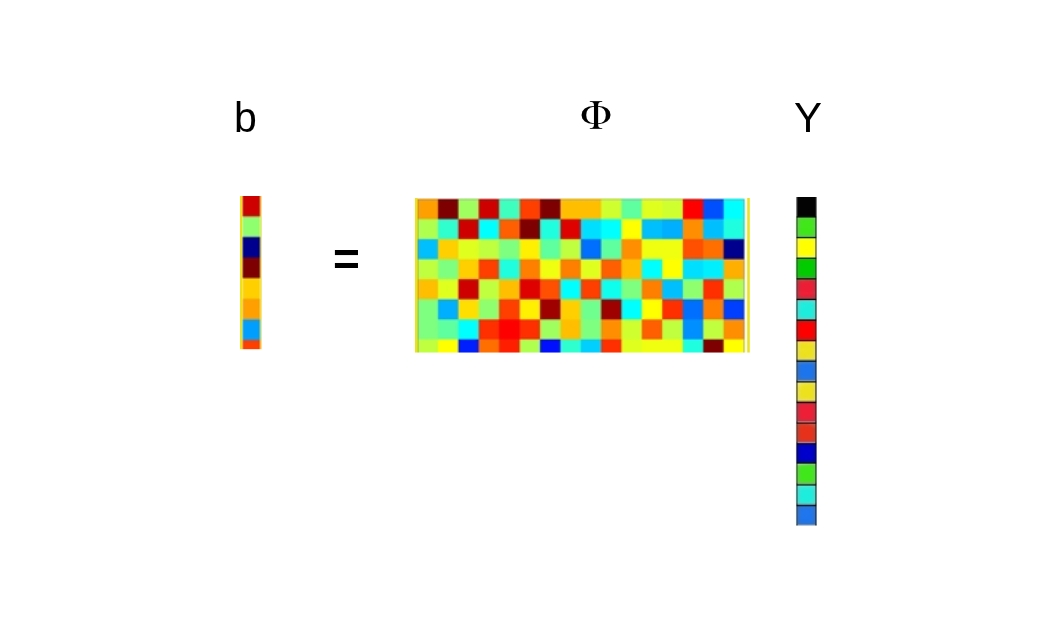
\includegraphics[height = 8cm, width=11cm]{figures/1}
    \caption{$ b= \Phi y$}
    \label{Figci1}
  \end{center}
\end{figure}

$\Phi$ is $M \times N$ matrix where $M<<N$.Now suppose we have $y= \Psi x$ where $x$ is a $k$-sparse representation of 
$y$ and $\Psi$ is the basis matrix. 
\newpage
\begin{figure}[!htbp]
  \begin{center}
      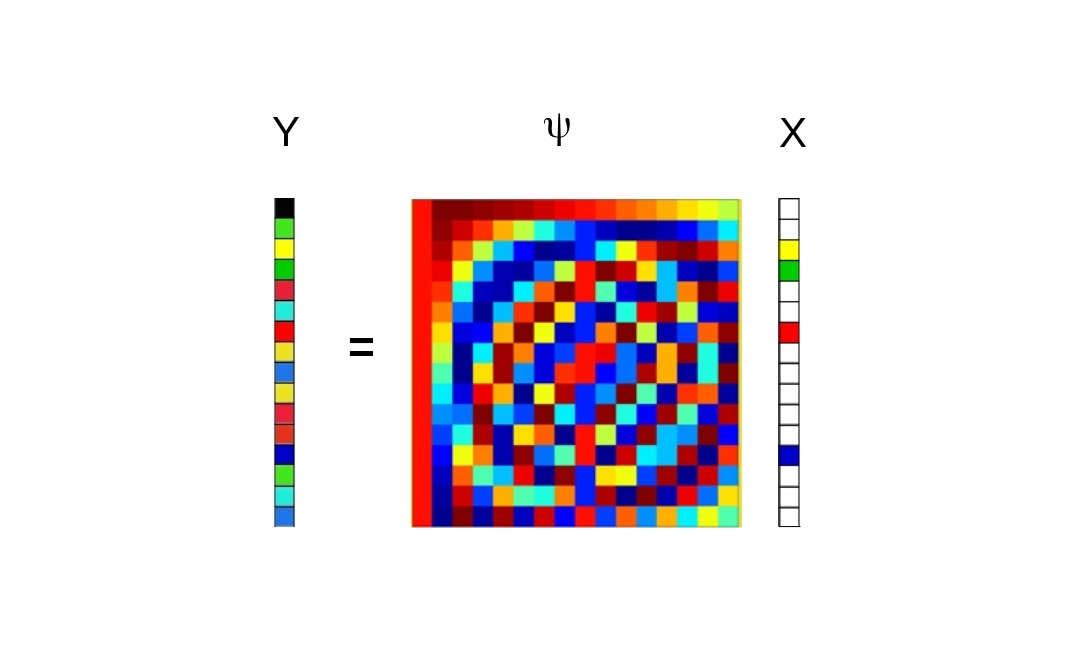
\includegraphics[height = 6cm, width=10cm]{figures/2}
    \caption{$ y = \Psi x$ }
    \label{Figci2}
  \end{center}
\end{figure}
The complete idea of compressed sensing is shown in following figure.

\begin{figure}[!htbp]
  \begin{center}
      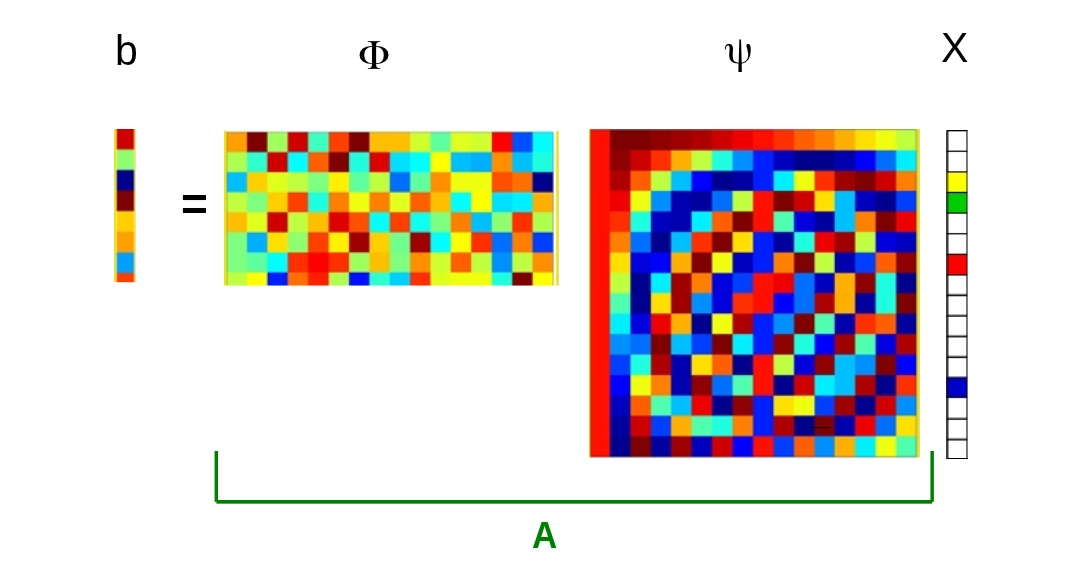
\includegraphics[height = 6cm, width=11cm]{figures/3}
    \label{Figci3}
  \end{center}
\end{figure}
In figure \ref{Figci3} equation $b = \Phi \Psi x$ is in $Ax = b$ form with $A = \Phi \Psi$.
Since $x$ is $k$-sparse, $x$ must be in one of the $C(n,k)$ subspaces of $R^N$. So if we have 
$m > k+1$ then exhaustive search can be done through these subspaces and we can determine which subspace $y$ belongs to.
This can be formulated as an optimization problem 

\begin{equation}
\mbox{minimize} \parallel x \parallel_{\ell_0} \mbox{subjected to }Ax=b
\label{1.2.1}
\end{equation}
where $\ell_0$ is the quasi-norm and is defined as 
\begin{equation}
 \parallel x \parallel_{\ell_0} =\displaystyle\sum\limits_{i=1}^{i=n}  I(x_i \neq 0) 
\label{1.2.2}
\end{equation}

where $I$ is an indicator function defined as 
\begin{equation}
I(x) =\left\lbrace
\begin{array}{lll}
  & 1 & x \neq 0\\
 & 0 & x = 0
\end{array}\right.
\label{1.2.3}
\end{equation}

\paragraph{}But performing this exhaustive search over all subspaces is computationally
intractable as $N$ increases (keeping $\alpha$ constant). One way of circumventing this problem is by using the $\ell_2$
norm as a proxy, which is equivalent to solving the following optimization problem. 

\begin{equation}
\mbox{minimize} \parallel x \parallel_{\ell_2} \mbox{subjected to }Ax=b
\label{1.5}
\end{equation}

\paragraph{}Solving the above equation leads to a solution for $Ax=b$ but it only guarantees $x$ to be small 
in the $\ell_2$ norm sense. In other words it does not help in reducing the number of non-zero components in the solution vector $x$ 
which is our prime aim.

%\begin{eqnarray}
%CIF: \hspace*{5mm}F_0^j(a) &=& \frac{1}{2\pi \iota} \oint_{\gamma} \frac{F_0^j(z)}{z - a} dz
%\end{eqnarray}
\nomenclature[zcif]{$CIF$}{Cauchy's Integral Formula}                                % first letter Z is for Acronyms 
\nomenclature[aF]{$F$}{complex function}                                                   % first letter A is for Roman symbols
\nomenclature[gp]{$\pi$}{ $\simeq 3.14\ldots$}                                             % first letter G is for Greek Symbols
\nomenclature[gi]{$\iota$}{unit imaginary number $\sqrt{-1}$}                      % first letter G is for Greek Symbols
\nomenclature[gg]{$\gamma$}{a simply closed curve on a complex plane}  % first letter G is for Greek Symbols
\nomenclature[xi]{$\oint_\gamma$}{integration around a curve $\gamma$} % first letter X is for Other Symbols
\nomenclature[rj]{$j$}{superscript index}                                                       % first letter R is for superscripts
\nomenclature[s0]{$0$}{subscript index}                                                        % first letter S is for subscripts

\paragraph{}Hence, minimizing the $\ell_0$-norm is computationally intractable and $\ell_2$-norm does not lead to sparse solutions.
A novel way of getting a sparse solution is by minimizing the $\ell_1$-norm subjected to $Ax = b$.

\begin{equation}
\mbox{minimize} \parallel x \parallel_{\ell_1} \mbox{subjected to }Ax=b
\label{1.6}
\end{equation}

\paragraph{}Solving this optimization problem leads to a sparse solution. It also guarantees the uniqueness in
solution as proved in .

\subsection{$\ell_1$ vs $\ell_2$}
\label{s:l1_vs_l2}

\paragraph{}One way of visualizing why $\ell_1$ leads to sparse solution and $\ell_2$ does not is shown in the 
following figure.

\begin{figure}[!htbp]
  \begin{center}
      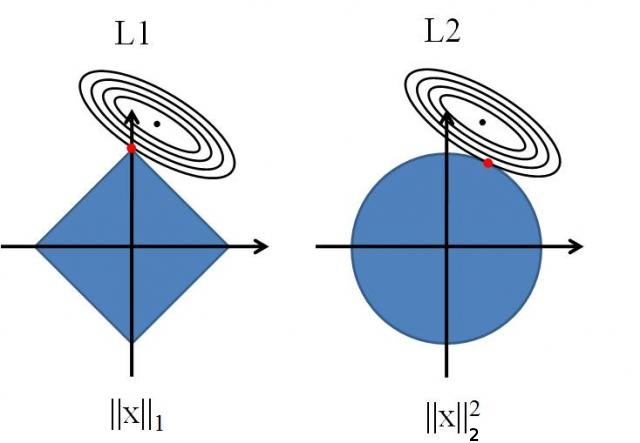
\includegraphics[height = 8cm, width=11cm]{figures/final_l1vsl2}
    \caption{$\ell_1$ vs $\ell_2$ ball}
    \label{Figl1vsl2}
  \end{center}
\end{figure}

\paragraph{}Figure (\ref{Figl1vsl2}) shows the $\ell_1$ ball and $\ell_2$ ball touching the contours of 
$\parallel Ax - b \parallel_{\ell_2}^2$. This clearly shows that due to the sharper corners of the $\ell_1$ ball,
contours of $\parallel Ax - b \parallel_{\ell_2}^2$ touch the $\ell_1$ ball at one of the axes, which is a sparse 
solution. However the $\ell_2$ ball is spherical and does not leads to a sparse solution.

\paragraph{}In general any $p$-norm is defined as 
\begin{equation}
 \parallel x \parallel_p = ( |x_1|^p + |x_2|^p + |x_3|^p +... |x_N|^p )^{\frac{1}{p}}
\label{1.7}
\end{equation}

\paragraph{}Further, an equivalent problem of minimizing the $p$-norm of $x$ is 
\begin{equation}
 minimize ( |x_1|^p + |x_2|^p + |x_3|^p +... |x_N|^p )
\label{1.8}
\end{equation}

\paragraph{}Let us compare the minimization of the $\ell_1$ norm and the $\ell_2$ norm. For the 
$\ell_2$ norm minimization, we care very little when $x_i < 1$ as compared to $\ell_1$ minimization because $\ell_2$ norm deteriorates
the smaller components more rapidly as compared to$ \ell_1$ norm. On the other hand 
during $\ell_2$ minimization we have a strong dislike when if $x_i > 1$. Hence, during minimization $\ell_2$
puts strong weights on larger components and a small weight (or zero weight) on smaller components of $x$ as
compared to the $\ell_1$ norm. So $\ell_1$ norm minimization places a larger emphasis on minimizing the smaller components
which in turn makes most of the components zero or approximately zero. This simple interpretation gives a clearer 
insight into why a solution of equation (\ref{1.6}) leads to sparse result. 

%Now I would like to cite the following: \cite{latex} and \cite{texbook}
%and \cite{Rud73}.

\subsection{Theorems for Compressed Sensing}
\label{s:cs_theorems}

\subsubsection{Restricted Isometry Property (RIP) or Uniform Uncertainty Principle (UUP)}

\paragraph{}UUP stands for “Uniform Uncertainty Principle“ (\cite{cand05}, \cite{cand07}). Matrices which follow these principle 
are called "UUP matrices". UUP matrices can compress vectors from high-dimensional space to low-dimensional space while
still being able to reconstruct these vectors. 

\paragraph{}In general, a $M \times N$ rectangular matrix $A$ is called orthogonal only if $M \geq N$ and each
column vector are orthonormal i.e. they all have unit length and are orthogonal to each other. Let 
$v_1, v_2 ... v_N$ be the '$N$' columns of $A$ matrix. Then
\begin{equation}
 v_i^*v_j   = 0 \hspace{10mm} \mbox{where } i \neq j \mbox{ and } i,j \mbox{ is from } 1 ... N
\label{1.9}
\end{equation}
\begin{equation}
 \parallel v_i \parallel_{\ell_2} = 1 \hspace{10mm} \mbox{where } i \mbox{ is from } 1 ... N
\label{1.10}
\end{equation}

\paragraph{}So this $A$ matrix can transform an $N$-dimensional vector $a =(a_1, a_2 ...a_N)$ to corresponding $M$ dimensional
vector, which is $ \displaystyle\sum\limits_{j=1}^{j=N} a_j v_j$. Now if this $A$ matrix is orthogonal, we know that norm 
of vectors are not changed when they are linearly transformed by an orthogonal matrix. So for above situation, we have
\begin{equation}
 \parallel \displaystyle\sum\limits_{j=1}^{j=N} a_j v_j \parallel_{\ell_2}^2  = \displaystyle\sum\limits_{j=1}^{j=N} |a_j|^2
\label{1.11}
\end{equation}

\paragraph{}This implies that $(a_1, a_2, ... a_N) \mapsto \displaystyle\sum\limits_{j=1}^{j=N} a_j v_j $ is an isometry i.e. 
given the encoded vector $ z = \displaystyle\sum\limits_{j=1}^{j=N} a_j v_j$ one can uniquely recover the original coefficients 
$(a_1, a_2 ... a_N)$. Furthermore, small changes in $z$ will not cause large fluctuations in $(a_1, a_2 ... a_n)$. Indeed, 
one can reconstruct the original coefficients quickly and explicitly by the formula 
\begin{equation}
 a_j = < z, v_j> 
\label{1.12}
\end{equation}

\paragraph{}But in the Compressed Sensing setting we cannot apply this property directly as we have $M << N$. In other words we 
cannot express a vector of say in '$t$' dimension with a basis vectors set of cardinality greater than $t$. So for our case

\begin{equation}
 a_1 v_1 + a_2 v_2 + ... +a_n v_N =0
\label{1.13}
\end{equation}
 
\paragraph{}If we can try to overcome the above restriction by weakening equation (\ref{1.11}) for all $(a_1,a_2, ... a_n)$ by
\begin{equation}
  (1-\delta_1)\displaystyle\sum\limits_{j=1}^{j=n} |a_j|^2 \hspace{3mm} \leq \hspace{3mm} \parallel \displaystyle\sum\limits_{j=1}^{j=n} a_j v_j \parallel_{\ell_2}^2  \hspace{3mm} \leq \hspace{3mm} (1+ \delta_2)\displaystyle\sum\limits_{j=1}^{j=n} |a_j|^2
\label{1.14}
\end{equation}
\paragraph{}where $\delta_1,\delta_2$ are constants such that $0 < \delta_1 \delta_2< 1 $. The above condition is as good
as saying columns of the matrix are locally orthogonal rather than globally perfectly orthogonal. Due to this property 
which is also called as \emph{Restricted Isometry Property (\cite{cand05, cand07})}, it turns out that one can pack more 
than $M$ vectors into $M$ dimensional space if one localizes the almost orthogonality condition so that it only holds for sparse sets of coefficients $(a_1,a_2, ... a_N)$. 
Sparsity parameter $k$ (less than $M$) plays an important role here. If we say that our sensing matrix $A$ obeys the UUP 
with sparsity $k$ then one has the almost orthogonality condition (\ref{1.14}) for any set of coefficients $(a_1,a_2, ... a_N)$, 
such that at most $k$ of the $a_j$ are non-zero. In other words, we only assume that any $k$ of the $N$ vectors $v_1, v_2,... v_N$
are almost orthogonal at one time. 

\paragraph{}Furthermore, constructing UUP matrices is an NP hard problem. In other words there is no polynomial 
time algorithm known which can construct these UUP matrices. The best possible methods are the one which could simply
search through all matrices in a given class and test each one of them for the UUP property. But this is an exponential-time
algorithm. However it has also seen that some matrices like random normalized Gaussian matrices, random normalized Bernoulli matrices are
UUP matrices. But they are all probabilistic in nature; in particular, these constructions are not 100\% guaranteed to actually produce
a UUP matrix, although in many cases the failure rate can be proven to be exponentially small in the size of the matrix. 
So for many larger scale applications it is actually exponentially less prone to failure.

\newtheorem*{mydefo}{Definition}
\begin{mydefo}
UUP matrices are the generalization of (rectangular) orthogonal matrices in which columns are locally 
almost orthogonal rather than globally perfectly orthogonal.
\end{mydefo}

\subsubsection{Incoherence}

\paragraph{}In Compressed Sensing we are dealing with two matrices $\Phi$ (sensing Matrix)
and $\Psi$ (Basis matrix which is used to represent $y$ in sparse basis). Coherence between the sensing
basis and Basis matrix defined as 
\begin{equation}
\mu(\Phi,\Psi) = \sqrt{N} max_{1\leq k, j\leq N} |<\Psi_k,\Phi_j>|
\end{equation}
\paragraph{}In simple words, coherence($\mu$) measures the largest correlation between two elements of $\Phi$ and $\Psi$. If
$\Phi$ and $\Psi$ contain correlated elements, then the coherence is large. Compressed Sensing is mainly concerned with
low coherence pairs i.e. we require low values of $\mu$. Classical example of incoherent basis pairs are the Fourier basis 
and Euclidean basis. These basis pairs are maximally incoherent with incoherence $\mu = 1$. Another example is pair of 
wavelets bases ($\Psi$) and noiselets $(\Phi$). The coherence between noiselets and Haar wavelets is $\sqrt{2}$ and 
between noiselets and Daubechies D4 and D8 wavelets, respectively, about 2.2 and 2.9. Noiselets are also maximally incoherent
 with euclidean basis and Fourier basis.

\paragraph{}Finally, random matrices are largely incoherent with any fixed basis $\Psi$. We select an orthobasis $\Psi$ 
uniformly at random, which can be done by orthonormalizing $N$ vectors sampled independently and uniformly on the unit 
sphere. Then with high probability, the coherence between $\Psi$ (Basis Matrix) and $\Phi$ (Sensing basis matrix) is 
$\simeq$ $\sqrt{2 logN}$. Random Gaussian i.i.d matrices also show very low coherence with fixed representation basis matrix $\Psi$.


\newtheorem{csth}{THEOREM (\cite{cand07})}
\begin{csth}
 Suppose $y \in R^N$ is sparse in some $\Psi$ basis and $x \in R^N$ is $k$-sparse representation of $y$. Now we select
$M$ measurements in $\Phi$ uniformly at random. Then if 
\begin{equation}
 M \geq C \mu^2(\Phi,\Psi)klogN
\end{equation}
for some constant $C$ the solution \ref{1.6} is exact with overwhelming probability.
\end{csth}

\paragraph{}The role of coherence is now clear; the smaller the coherence, the fewer samples are needed,
hence compressed sensing require low coherence pairs of basis matrices. One suffers no information loss by measuring just
about any set of $M$ coefficients which may be far less what the signal size apparently demands. If $\mu(\Phi,\Psi)$ is equal or
close to one, then of the order of $klogN$ samples suffice instead of $N$.

\subsection{Applications}
\label{s:cs_applications}
The fact that sparse signals can be reconstructed efficiently using very few number of incoherent
samples which is proportional to sparsity ($k$) has far reaching implications and applications. The main 
areas where compressed sensing had proven itself as a more advantageous and efficient technique are
\begin{itemize}
 \item \emph{Data compression}. In some situations, the sparse basis $\Psi$ may be unknown at the encoder or impractical to implement
for data compression. However a randomly designed $\Phi$ can be considered a universal encoding strategy, as it need not be 
designed with regards to the structure of $\Psi$. This universality may be particularly helpful for distributed source
coding in multi-signal settings such as sensor networks (\cite{baron09}).
 \item Channel coding. Compressed Sensing principles can be turned around and applied to design fast error correcting codes over
the reals to protect from errors during transmission (\cite{cand05}).

 \item \emph{Inverse problems}. The only way to acquire $x$ may be to use a measurement system $\Phi$ of a certain
    modality. However, assuming a sparse basis $\Psi$ exists for $x$ that is also incoherent with $\Phi$, then efficient sensing will
    be possible. One such application involves MR angiography and other types of MR setups, where $\Phi$ records a
    subset of the Fourier transform, and the desired image $x$ is sparse in the time or wavelet domains (\cite{lustig06}).

 \item \emph{Data acquisition}. Finally, in some important situations the full collection of $N$ discrete-time samples of an analog signal
may be difficult to obtain (and possibly difficult to subsequently compress). Here, it could be helpful to design physical
sampling devices that directly record discrete, low-rate incoherent measurements of the incident analog signal.

\end{itemize}
